\section{\textbf{Project Title 1}}
\subsection{Introduction}
\lipsum[12]

\textbf{An example of citation \cite{muokEngineeredChemotaxisCore2020,briegelMobilityTwoKinase2013}}.

\begin{figure}[H]
    \centering
    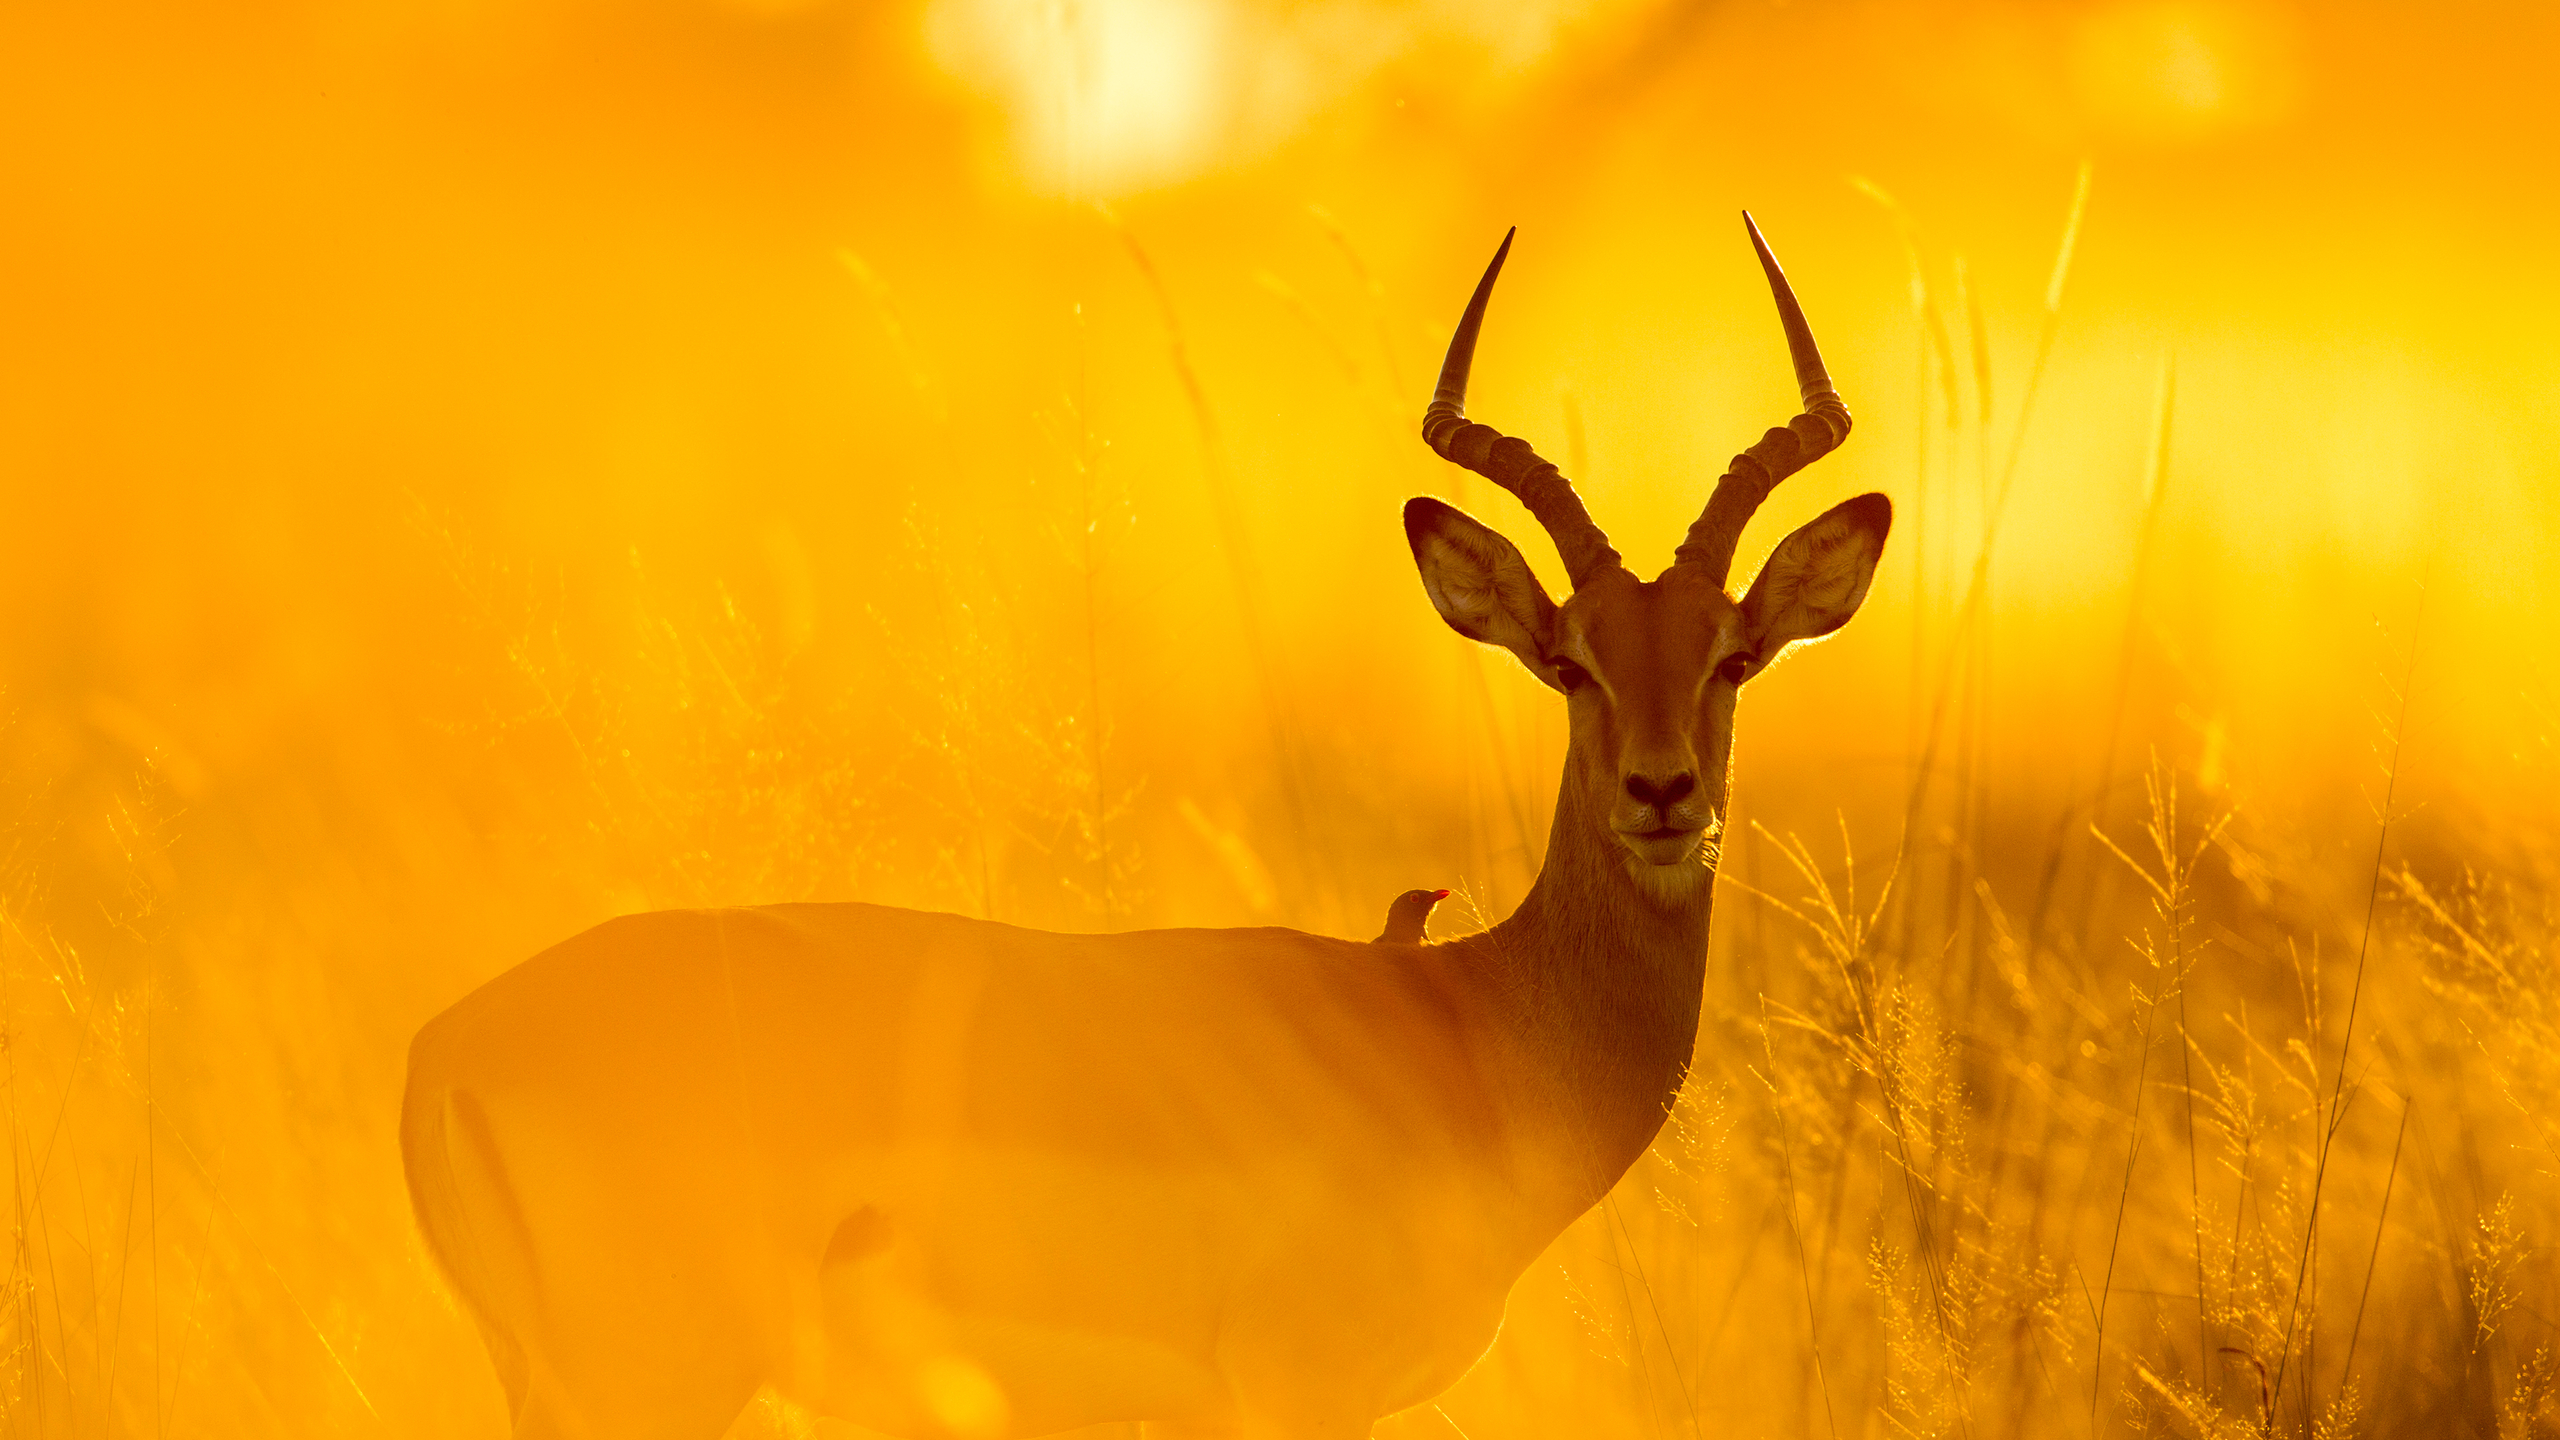
\includegraphics[width=400pt]{assets/figures/OrangeImpala.jpg}
    \caption{A placehold for figure captions}
    \label{fig:label1}
\end{figure}


\subsection{Methods}
\textbf{A simple example of enumerated list}
\begin{enumerate}
    \item \lipsum[13]
    $$
    f(x) = A \sin(x) \exp(\frac{1}{(x - \delta)^2})
    $$
    \item \lipsum [2]
\end{enumerate}


\subsection{Results}
\lipsum[15]

\begin{table}[H]
    \centering
    \caption{Fake data example}
    \begin{tblr}{
      colspec = {lcc},
      row{1} = {font=\bfseries}
    }
      \hline
      Name     & Value & Category \\
      \hline
      Alpha    & 12.3  & A \\
      Beta     & 45.6  & B \\
      Gamma    & 78.9  & C \\
      \hline
    \end{tblr}
  \end{table}

\subsection{Future Plans}
\lipsum[20]

\textbf{An example of enumerated list with subtitles:}
\begin{description}[style=nextline,labelindent=0.5cm]
    \item[1. Argument or conclusion] \lipsum[17] 
    \item[2. Argument or conclusion] \lipsum[18]
\end{description}


\newpage